{Plot the points with the given polar coordinates.

\noindent\begin{minipage}[t]{.5\linewidth}
\begin{enumerate}
	\item $A=P(2,0)$
	\item	$B=P(1,\pi)$
\end{enumerate}
\end{minipage}
\begin{minipage}[t]{.5\linewidth}
\begin{enumerate}\addtocounter{enumii}{2}
	\item $C=P(-2,\pi/2)$
	\item	$D=P(1,\pi/4)$
\end{enumerate}
\end{minipage}
}
{\begin{minipage}[m]{\linewidth}
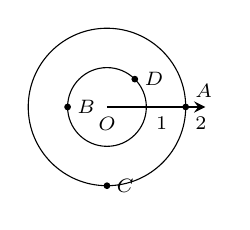
\begin{tikzpicture}[scale=.5]
	\foreach \x in {1,2}
	{\draw (0,0) circle (\x);
		\draw (\x,0) node [below right] {\scriptsize $\x$};
	}
	\draw [thick,->,>=stealth] (0,0) node [below] {\scriptsize $O$} -- (2.5,0);
	\filldraw (xyz polar cs: angle=0,radius=2) circle (2pt) node [above right] {\scriptsize $A$}
	      (xyz polar cs: angle=180,radius=1)circle (2pt) node [right] {\scriptsize $B$}
				(xyz polar cs: angle=90,radius=-2)circle (2pt) node [right] {\scriptsize $C$}
				(xyz polar cs: angle=45,radius=1)circle (2pt) node [right] {\scriptsize $D$};
	\end{tikzpicture}
	\end{minipage}
	}
